%===========================================
%                                      NOTES
%===========================================
% R code to generate correlation matrix and tables is in 'Bounce.R'

%===========================================
%  TITLE: VARIATION IN MUTATIONAL PARAMETER ESTIMATES
%===========================================
\chapter{Variation in mutational variance-covariance matrices for \textit{Drosophila serrata} wing shape across sequential generations}
\vspace{2cm}

\section{Abstract}
Robust estimation of how mutations contribute to phenotypes is central to evolutionary biology and depends on understanding the pattern and extent of mutational pleiotropy between traits. Extensive mutational pleiotropy may constrain evolution; however, if utilised in experimental design, can provide a method of improving detection of mutational effect.  Here, I estimate $\vec{M}$, the mutation covariance matrix, for six functionally related \textit{Drosophila serrata} wing shape traits, where I expect pleiotropy to be pervasive. Through the application of two population size treatments to lines that had previously undergone mutation accumulation (MA), I address the impact of increasing levels of selection on the magnitude and orientation of $\vec{M}$. By phenotyping for six consecutive generations (in both treatments), I could simultaneously determine how variation due to environmental heterogeneity (time-points) influenced $\vec{M}$. Employing several approaches for comparing matrices, I found a trait combination ($m_{max}$) associated with non-zero mutational variance across all 12 population samples (two treatments by six generations). Matrices were found to not diverge along $m_{max}$, where differences were transient. I discuss the implications of my results for improving estimation of mutational variance and the relative constraints that mutation has for wing shape evolution. \par

\newpage
%%%===========================================
%%%                                         INTRO
%%%===========================================

\section{Introduction}

Understanding how spontaneous mutations affect the phenotype is central to both evolutionary and biomedical issues, including extinction risk \citep{Land94, lync95,Loew06}, the maintenance of quantitative genetic variance \citep{Burg00, John05}, and the nature of complex human disease \citep{John20}. Measured as the per-generation variance due to new mutation ($V_M$), there has been a substantial effort devoted to estimating this parameter \citep[][Chapter 12]{Houl96, Hall09, Wals18c12}, yet comparatively less attention has been applied to the mutational association between traits \citep{Jone03,Jone07,Este06}. The relative magnitude of $V_M$ in traits and the efficacy of mutation-selection processes acting upon $V_M$, will depend on the level and nature of covariation between traits. \par
Mutational covariation between traits reflects patterns of pleiotropic allelic effects and linkage disequilibrium between multiple mutations \citep{Land80,Falc96,Phil06}. Covariation due to linkage is expected to erode rapidly over time \citep{Land80}, consequently pleiotropy via naturally occurring mutation has greater implications for generating and maintaining standing genetic variation in natural populations \citep{John05}. Estimates of mutational variance (diagonals) and covariance (off-diagonals), as M-matrices, have previously been obtained in lines with induced mutations \citealp{Cama00, Keig00} or spontaneous mutations \citep[e.g.,][]{Houl94, Este04,Mall23}. Generally, strong positive correlations between life history traits are reported \citep{Houl94, Keig00,Este06}; a phenomenon unanticipated in traits such as early versus late fecundity where antagonistic pleiotropy due to senescence was predicted \citep{Houl94}. While a difference between mutational and standing genetic trait covariances may reflect the action of selection \citep{Este06}, for traits with consistently biased direction of mutational effects \citep[i.e., mutations typically decrease fitness:][]{Hall09} linkage may cause a transient pattern of positive correlations \citep{Keig00}. The inflated rate of mutations in mutagenesis studies potentially causes statistical association between traits as the likelihood of sampling multiple deleterious mutations is increased. Similarly, in mutation accumulation (MA) studies, deleterious mutations may accumulate to varying degrees within each line, also resulting in a linkage effect that produces widespread correlations between traits \citep{Keig00}. \par

For non-fitness traits, for which mutations do not appear to have biased directional effects, linkage among mutations is not predicted to generate covariance. The opportunity for pleiotropy to generate patterns of among-line mutational covariance will depend on the average correlation of pleiotropic effects among traits. Drosophila wing phenotypes have emerged as a model for studying genetics and evolution \citep{Meze05,Houl17}. Wing phenotypes are expected to share a genetic basis and developmental pathways \citep{Meze05, Neto09}, where functionally related traits (e.g. different measures of a body region) might be precisely the context in which we expect pleiotropy to be pervasive. Estimates of mutational covariance among wing traits in \textit{D. melanogaster} \citep{Houl13,Houl17} and \textit{D. serrata} \citep{Duga21} suggest that mutation does typically generate strong covariance among shape traits, and that this covariance persists in standing genetic variation. If there is a strong bias in the distribution of pleiotropic effects of mutations, such that a single combination of traits is associated with mutational variance ($m_{max}$), then other trait combinations will experience limited introduction of genetic variance creating nearly null spaces that potentially constrains evolution \citep{Gomu09,Houl13, Hine14}. In their study, \citet{Houl17} concluded that due to the similarity in orientation between the mutational, standing genetic and the divergence matrix (that embodied 40 million years of \textit{Drosophila} wing differentiation), that mutation could predict the trajectory of long-term phenotypic evolution \citep[also see][]{Farh15}.\par

Patterns of covariance between traits can arise from processes other than pleiotropic mutation, where the interpretation of $\vec{M}$ can be obscured if unaccounted for. Estimating quantitative genetic variances and covariances requires large sample sizes \citep{Klei73,Klei74,Lync98c21}, and often entails laboursome phenotyping techniques as labour-saving high-throughput methods are not well established \citep{Houl10}. Sampling error can generate strong covariance among variables, particularly when the number of independent samples is small relative to the number of variables \citep{John07, Blow15,Szte17a}. Similarly, micro-environmental sensitivity (e.g., varying culture conditions or larval competition) may also inflate estimates of mutational covariances, as larger mutational variances are associated with reduced phenotype canalization and vice versa \citep{Stea95,Zhan05env, Baer08}. Environmental effects are expected to act on phenotype in the same direction as genetic (mutational) covariances, inflating within line variance, as both often share the same developmental and biochemical pathways \citep{Chev84}. However, both technical sampling error and micro-environment variance should be independent in each generation, where repeated sampling will improve the detection of mutational (co)variance.\par

Here, I utilise the same repeated-sampling experimental design as described in Chapter 2, coupled with multivariate analyses of six wing shape and size traits, to address three main questions: 1) can multivariate analyses of functionally related sets of traits provide a better estimation of mutational variance compared to univariate estimates; 2) does the opportunity for selection in the short term alter the genetic covariance among traits produced by mutation, and 3) do sampling error or micro-environmental variation cause trait covariances that reflect mutational covariances. When mutation has pleiotropic effects across the measured traits, this shared variation will be captured by a single linear combination of traits, the first eigenvector of $\vec{M}$. To assess if this shared variation increases the power to estimate mutational variance, I will compare the statistical support for variance in the eigenvectors of $\vec{M}$ to the statistical support for variance in the individual traits (as reported in Chapter 2). I will then use tensor analyses to compare different estimates of $\vec{M}$, reflecting differences in either opportunity for selection or opportunity for micro-environmental effects. These analyses characterise the nature of any differences between the $\vec{M}$. \par

% %===========================================
% %                                         METHODS
% %===========================================
\section{Methods}
\subsection{Population history and wing data collection}
The mutation accumulation (MA), population size manipulation and wing data collection are detailed in Chapter 2. Briefly, I used a single \textit{D. serrata} Reference Genome Panel (DsRGP) line \citep{Redd18} as a progenitor, establishing 200 MA lines that were maintained for 20 generations by single brother-sister pairs. From these MA lines, 42 were randomly selected and expanded to found two sublines: a small (S: $N = 24$ flies per line) and large (L: $N = 288$) population size treatment, which were maintained for a further six generations. To ensure comparable larval environments across sublines, each treatment consisted of a foundation experimental unit of 12 male and 12 female parents per vial each generation, where more vials were included to make up the L treatment. For the S treatment, a single vial was used to propagate each line; however, to estimate within-line variation, a replicate vial was maintained at each generation but did not contribute offspring to the next generation. The L population consisted of twelve vials per line, where offspring were pooled across all vials, within a line, before virgins were collected to found the next generation.\par

A total of 5,135 wings from male flies were available for analyses, sampled from the six generations, 84 sublines and two emergence vials from each subline, two haphazardly chosen vials in the L treatment, and from the focal and replicate vial for the S treatment lines. Nine wing landmark positions were aligned using a generalised Procrustes least squares super imposition \citep{Rohl07}. From the resulting aligned X-Y coordinates for each landmark, inter-landmark distances (ILDs) were calculated. A subset of six traits (wing size and five ILDs) were chosen for analysis; this subset of traits had non-zero estimates of among-line variance in all six generations for both treatments (see Chapter 2, Figure~\ref{fig:Fig5VlBounce}), and relatively low trait covariances, ensuring that multicollinearity did not preclude model convergence, and that asymptotic matrices were positive definite (supporting estimation of informative confidence intervals). Reflecting differences in collinearity among ILDs across different studies of the same species, the six analysed ILDs differ from sets of ILDs previously used to describe wing shape in \textit{D. serrata} \citep{McGu13, McGu15}. Prior to analysis, Mahalanobis distance, estimated across six traits, was used to identify multivariate outliers (above a critical value of $\chi^2 = 22.46, \alpha =0.01$; 55 outliers across the 5135 flies, $< 1.1$\%). To facilitate convergence in multivariate models, data for each trait was variance standardised (mean = 0, standard deviation = 1) across all generations and treatments.\par

\subsection{Estimating mutational variance-covariance matrices}
To investigate the effects of mutation-selection-drift (captured by my two population size treatments) and random environmental effects on the repeatability of the estimate of mutational (among-line) variance and covariance matrix I estimated the 12 (two treatments measured in six generations) among-line ($\vec{M}$) and residual ($\vec{R}$) covariance matrices for my six traits, using restricted-maximum likelihood (REML) in PROC MIXED in SAS v9.4 (SAS Institute Inc., Cary, NC.) to fit:

\vspace{-\parskip}
\begin{equation}
y_{ijklm} = \mu + Line_{k(j)} + Vial_{l(ijk)}+ \varepsilon_{ijklm} \label{eqn:multi_1}
\end{equation}
\noindent where $y_{ijklm}$ was the vector of six trait values for the $m^{th}$ wing, for the $l^{th}$ vial, within the $k^{th}$ line, for the $j^{th}$ treatment in the $i^{th}$ generation. The mixed model fit the vector of overall means per trait ($\mu$). The random effects of the model partitioned the variation at the among-line (Line) and the within-line, among-replicate rearing vial (Vial) level, while the residual error ($\varepsilon$), estimated the variance among individual flies within a rearing vial. I modelled unstructured variance-covariance matrices for each random effect. To place confidence intervals about my estimates of the variance components, I generated a parametric sampling distribution using an asymptotic approximation of the covariance parameter estimates, applying the REML-MVN method developed by Meyer and Houle \citeyear{Houl15,Meye13}. The distribution was obtained by sampling from $N\sim(\boldsymbol{\hat{\theta}}, \vec{V})$ 10,000 times, where $\boldsymbol{\hat{\theta}}$ was the vector of observed covariance parameter estimates, and $\vec{V}$ was the asymptotic variance-covariance matrix \citep{Houl15,Meye13,Szte17a}. \par

\subsection{Comparing mutational variance-covariance matrices}

I employed three geometric approaches to investigate changes in the variances and covariances of my matrices. First, I used Krzanowski's subspaces method \citep{Krza79, Agui14}, to determine if the 12 populations, differing in their opportunity for mutation, drift and selection, retained the same multivariate axes of mutational (residual) variance. Second, I used a covariance tensor analysis to determine the trait combinations in which the populations differed the most. These two approaches are similar in that they both consider how genetic (mutational) variance is distributed among populations in multivariate space, but do not directly explore how stable these matrices are over time or whether the covariance structures differ. To address this, the third approach used \citet{Mitt09}’s relative genetic distance to explore how matrices diverge through time and across varying levels of selection.\par

For each of the two treatments in each of the six generations, I first characterise axes of shared wing shape variation among populations using Krzanowski’s subspaces method \citep{Krza79, Agui14}. Considering each of my two treatments in each of my six generations as 12 independent populations, I identify the shared subspaces across the 12 among-line,  $\vec{M}$, covariance matrices using \citep{Krza79}:\par

\vspace{-\parskip}
\begin{equation}
\vec{H} = \sum_{t=1}^{p} \vec{L}_t^{T}\vec{L}_t \label{eqn:multi_2_H}
\end{equation}

\noindent where $\vec{L}_{t}$ contains the subset of the $j$th largest eigenvectors, as rows, of $\vec{M}$, (and $\vec{L}_{t}^{\vec{T}}$ its transpose containing eigenvectors as columns), $p = 12$ (the number of populations to be compared. The number of eigenvectors included for each $\vec{M}$ was determined as $j = \frac{n}{2}$; $n$ = number of traits; here $j = 3$. Using more eigenvectors than half of the number of traits (i.e. $j >  \frac{n}{2}$) limits the ability to uncover distinct informative dimensions, as when $j = n$ the subspaces would completely overlap each other \citep[further explanation given by][]{Blow04}. These $j$ eigenvectors represent at least 90\% of genetic variance in each $\vec{M}$ (see Results). $\vec{H}$ was determined by implementing the EvolQG v.0.2-6 \citep{Melo15} package in R. Spectral decomposition of $\vec{H}$ describes the degree of shared variance across the different populations, where the eigenvalues are interpreted on a scale of 0 to $p$; here, an eigenvalue of 12 would indicate that all 12 populations have variance in the direction of the associated eigenvector.\par 

I complimented the Krzanowski analysis, with a fourth-order covariance tensor analysis, which identifies directions of trait space in which populations differ in variance \citep{Hine09, Agui14}. By using a covariance tensor, I was able to describe independent aspects of variation in the covariance structure across the 12 M among-line matrices and, separately, the 12 R residual matrices. Here I describe the tensor method focusing only at the among-line covariance matrices; however, this sequence of analyses was similarly applied to the residual matrices. First, the fourth-order $\Sigma_{\vec{M}}$ was mapped onto the second-order symmetric S matrix that has a dimension of $\frac{n(n+1)}{2}$ where $n$ is the number of traits. The $\vec{S}$ consists of four quadrants, where the upper left quadrant contains the variances of the variances on the diagonal and the covariances of the variances on the off-diagonal. The lower right quadrant diagonal elements are the variances of the covariances, and the off-diagonal elements are twice the covariances of the covariances. The two remaining quadrants are reflections of each other, where the elements are the product of the square-root of two multiplied by the covariances between the variance and covariance of the original $\vec{M}$. Eigenanalyses of $\vec{S}$ results in eigenvalues and $k$ $n \times n$ eigentensors ($\vec{E}_k$, in unarranged vector form), which capture independent differentiation in variances and covariances among the M matrices. To place confidence intervals on the eigentensor eigenvalues, I used the REML-MVN framework. For each $i^{th}$ ($i=1,$...10,000 as described above) set of 12 $\vec{M}$, I determined the $\vec{S}_i$. I then projected the 1:$k^{th}$ eigenvectors of $\vec{S}$ (the unarranged elements that form the $k^{th}$ $n \times n$ eigentensor, $\vec{E}_k$) onto each $\vec{S}_i$, to generate the posterior distribution for each $\vec{E}_k$.\par

To understand how the genetic variance in my 12 matrices diverge along the independent axes captured by each eigentensor, I determined the coordinates for each $\vec{M}$. To do so, it must first be appreciated that each $p^{th}$ population of $\vec{M}$, can be expressed as a linear combination of the  $k^{th}$ eigentensor;\par

\vspace{-\parskip}
\begin{equation}
\vec{M}_p= \sum_{k}C^{p,k}\vec{E}_k \label{eqn:multi_3_cord}
\end{equation}


\noindent where, the coordinates $C^{p,k}$ are calculated as the Frobenius inner product of $\vec{E}_k$ and $\vec{M}_p$ \citep{Hine09}. Similar coordinates between $\vec{M}$ indicate that their mutational variance, combined across all traits, does not differ in the direction captured by the given eigentensor. $\vec{M}$ with the largest absolute values of the coordinates contribute strongly to the differences between matrices, and opposing signs contribute in opposing directions. By assessing the coordinates of each eigentensor for each $\vec{M}$, I was able to determine the level of genetic variance captured by each eigentensor in each of the 12 $\vec{M}$. I similarly examined the coordinates of my among-line eigentensors $\vec{E}_k$ in the space of the $\vec{R}_p$ matrices, to determine whether each eigentensor was associated with proportional residual variance.\par

To facilitate the interpretation of the information captured by my eigentensors, I used further eigenanalysis, to reduce each eigentensor into its eigenvalues and eigenvectors. The eigenvalues represent the spread of genetic covariance represented by the eigentensors, and consequently, can be both positive and negative, where the absolute value reflects the magnitude of the contribution of that independent eigenvector to the difference in variance captured by that eigentensor. To determine if a particular treatment or generation generated the majority of among-line (residual) variance in the associated direction, the $i$th eigenvector ($e$, $i = 1,..., n$) from the $k$th eigentensor was projected through each of the 12 $\vec{M}$ ($\vec{R}$) to estimate the among line variance (residual variance) associated with that direction \citep{Hine09}: 

\vspace{-\parskip}
\begin{equation}
V_L= e_{k,i}\vec{M}[e_{k,i}]^{T} \label{eqn:multi_4_vlprj}
\end{equation}

\noindent This projection was done for the set of eigenvectors that accounted $\sim 90\%$ of the variance in that eigentensor. However, it is important to note that while eigenvectors within an eigentensor are independent from another, eigenvectors across eigentensors are not independent, a characteristic that becomes apparent across my set of major eigentensor eigenvectors (see Results). That is, this estimated variance may be shared across different eigentensors.\par

Finally, I used \citet{Mitt09}'s relative genetic distance to determine how my 12 $\vec{M}$s diverged. This method was initially devised to explore ontogenetic change, where shared developmental pathways contribute disproportionately to the same phenotypic traits as organisms age; such patterns can be revealed by tracking unique change in each covariance matrix relative to the other matrices \citep{Mitt09, Book14}. This method can similarly be applied here to determine how levels of mutational pleiotropy (covariance) varies across generations. This method utilises the Riemannian manifold, a metric that measures the length of the shortest geodesic curve between two matrices and requires the covariance matrix to be positive-definite \citep{Mitt09}. I was precluded from exploring how the $\vec{M}$s diverged in the space of the first two eigentensor eigenvectors ($e_{11}$ and $e_{16}$) as one of the 12 resulting matrices was not full rank. Instead, I calculated the distances in the space of the first three eigenvectors of Krzanowski’s subspace ($h_1$, $h_2$ and $h_3$, see Results below). Using Equation 2 from \citet{Mitt09}, each distance was calculated as:\par

\vspace{-\parskip}
\begin{equation}
d_{cov}(\vec{M}_a, \vec{M}_b) = \sqrt{ \sum_{i=1}^{n}(log \lambda_{i})^{2}}  \label{eqn:multi_5_mitte}
\end{equation}

\noindent where $\vec{M}_a$ and $\vec{M}_b$ are a pair of my 12 M matrices, and $\lambda_i$ was the eigenvalue of the relative eigenvalues of $\vec{M}_a$ with respect to $\vec{M}_b$, or more exactly, the eigenvalues of the ratio of one matrix to the other ($\vec{M}_a^{-1}\vec{M}_a$) \citep{Mitt09}. Each value of $d_{cov}(\vec{M}_a, \vec{M}_b)$ was then used as an element within the symmetrical relative distance matrix, $\vec{D}$;\par

\begin{equation}
\vec{D} =
\begin{pmatrix}
0 & d_{cov}(\vec{M}_1, \vec{M}_2) & \cdots & d_{cov}(\vec{M}_1, \vec{M}_{12})\\
d_{cov}(\vec{M}_2, \vec{M}_1) & 0 &  \cdots & d_{cov}(\vec{M}_2, \vec{M}_{12})\\
\vdots  & \vdots  & \ddots & \vdots  \\
d_{cov}(\vec{M}_{12}, \vec{M}_1) & d_{cov}(\vec{M}_{12}, \vec{M}_2) & \cdots  &0
\label{eqn:multi_6_D}
\end{pmatrix}
\end{equation}

\noindent As there would be no difference between a matrix and itself, the diagonal elements of $\vec{D}$ equal to zero. I performed a principle coordinate analyses of $\vec{D}$, using the \textit{vcvComp} v1.0.2 package in R \citep{LeMa19}. The principal coordinate analysis is an eigen-decomposition of the $\vec{D}$, that transforms the high-dimensional, non-linear space of $\vec{D}$ into a low-dimension ordination (of $p-1$ dimensions, where $p$ is the number of matrices, here 12), that is easier to assess differences in variance-covariance structures over time. \par


%%===========================================
%%                    RESULTS
%%===========================================
\section{Results}

I observed relatively similar magnitude of mutational variance across the 12 populations (Figure~\ref{fig:multi_specM}A). Consistent with the robust support for mutational variance in each individual trait (Chapter~2), I observed the lower 90\% confidence interval of the trace (sum of individual trait variances) of each of the 12 among-line six-trait M matrices to be substantially above zero (Figure~\ref{fig:multi_specM}A). Spectral decomposition of each of the 12 matrices showed that the first eigenvector explained an average of 63\% of the among-line variance in a population (generation $\times$ treatment), with a sharp decay in the variance of subsequent eigenvectors (white boxplots, Figure~\ref{fig:multi_specM}B). The first eigenvalue was substantially greater than the largest individual trait variance within a matrix (grey boxplots, Figure~\ref{fig:multi_specM}B), suggesting the presence of shared mutational variance among traits within each population. Looking at the individual eigenvalues, it was notable that the large population had more eigenvalues with positive CI (e.g., four in generation six, Table~\ref{tab:multi_Meigvals}) than the small (at most first three, Table~\ref{tab:multi_Meigvals}). Sampling error can upwardly bias eigenvalues (and their REML CI) \citep{Szte17a}, but here, with consistent sample sizes in both the large and small population size treatments, I expect sampling error to consistently affect both treatments (Table~\ref{tab:multi_suppdatDist}). Therefore, this observation may suggest that the different opportunities for mutation-selection-drift have impacted my power to detect among-line variance. \par

The amount of total residual (among individual) variance in each of the 12 $\vec{R}$ were an order of magnitude greater than the mutational variance in the M matrices (Figure~\ref{fig:multi_specR}A). Pronounced temporal pairing of residual estimates across treatments suggests that my experimental design ensured individual flies experienced comparable microenvironments (e.g., larval competition, Figure~\ref{fig:multi_specR}A). However, estimates differed across generations, with the greatest difference between the third and fourth generation, resulting in ~20\% reduction in residual variance. In contrast to $\vec{M}$, spectral decomposition of the residual covariance matrices, $\vec{R}$, suggested relatively little shared variance among traits, where the first eigenvector only accounted for an average of 35\% of the residual variance, followed by an average of 23\% in the second eigenvector (Figure~\ref{fig:multi_specR}B). In all six dimensions of the R matrices, in each treatment, for every generation, the CI intervals did not overlap zero (Table~\ref{tab:multi_suppRmat}, indicating that the residual variances were capturing independent random sampling error. \par

\subsection{Common subspaces}

I observed extensive idiosyncratic patterns for each individual trait (univariate analyses Chapter 2, Figure~\ref{fig:Fig5VlBounce}) suggesting that the mutationally variable trait combinations (i.e., eigenvectors of $\vec{M}$) might differ among populations. The Krzanowski’s subspace analysis strongly suggests that there was at least one axis of mutational variance shared among all populations. The first eigenvector, $h_1$, of the subspace, $\vec{H}$, had an eigenvalue that was 11.68 (Table~\ref{tab:multi_Heigvals}), very close to the maximum possible value of 12 (equally shared across all 12 $\vec{M}$); and most likely represents the major axes of mutational variance accumulated during the MA experiment, prior to founding the large and small population size treatments. This vector was characterised by a strong positive loading for ILD3.7 (0.57), the length of the distal wing area (Figure~\ref{fig:multi_WingNineLM}, and a strong negative loading for ILD1.5 (- 0.68), the wing depth (Figure~\ref{fig:multi_WingNineLM}, Table~\ref{tab:multi_Heigvals}), consistent with mutation generating variation along an axis of short and wide versus long and narrow wing shape. \par

While all 12 populations retain some variation along $h_1$, the amount of variance may differ. To assess this, I projected $h_1$ through each $\vec{M}$. The magnitude of variance was similar across all populations, with only the generation 3 estimate from the big population size treatment appearing to have a slightly different (elevated) variation in this direction (Figure~\ref{fig:multi_HvecsThruMnR}A). I next projected $h_1$ through each $\vec{R}$, establishing whether the major axis of shared mutational variance accumulated proportional micro-environmental variation. Although there was a moderate positive correlation between the mutational and residual variance captured by $h_1$, the null hypothesis of no association was not rejected ($r = 0.42$, $P = 0.18$; Figure~\ref{fig:multi_HvecsThruMnR}G). The magnitude of residual variance accounted by $h_1$ differed across generations but not treatment; suggesting that the micro-environment similarly affected the treatments (Figure~\ref{fig:multi_HvecsThruMnR}D). \par

The second subspace axis, $h_2$, appears common to at least some matrices with an eigenvalue of 9.47. Most (all except the third) generations of the large population had substantial mutational variance along $h_2$ whereas only two generations in the small population (second and fifth) varied along this axis (Figure~\ref{fig:multi_HvecsThruMnR}B). Notably, centroid size was the single dominating loading for $h_2$ (0.89, Table~\ref{tab:multi_Heigvals}); indicating that there was potentially more independent mutational variance for size in the large than the small population. The third axis $h_3$ ($\lambda = 7.59$), seems to detect transient mutational variance comparably across treatments, with no temporal trends (Figure~\ref{fig:multi_HvecsThruMnR}C). For both $h_2$ and $h_3$, there was no evidence that residual variance proportionally varied in these directions (Figure~\ref{fig:multi_HvecsThruMnR}H and I).\par

\subsection{Differences in $\vec{M}$}
Krzanowski’s subspace analysis revealed that not all axes (eigenvectors) of mutational variance were shared among the 12 $\vec{M}$. To further investigate how my matrices diverged, I applied a tensor analysis. In contrast to the median trace for the 12 $\vec{M}$ (0.65), the median among-line variance accounted by the 11 possible non-zero eigentensor eigenvalues was two orders of magnitude smaller at 0.004 (Figure~\ref{fig:multi_TwoEigTen}A). This indicates that the difference in variance was a very small component of the total variance in each $\vec{M}$. The limited amount of variance captured by the eigentensors potentially poses a problem when generating posterior distributions to estimate confidence intervals. In Figure Figure~\ref{fig:multi_TwoEigTen}A, my eigentensor
eigenvalues CIs are asymmetric, consistent with eigenvalue sampling distributions conforming to a Marchenko-Pastur (MP) distribution (\citealt{Blow15}; but see \citealt{Agui14} Figure 4 for an eigentensor example). However, in some cases, my estimates fall below their REML-MVN CIs. This is most likely due to sampling error, resulting in overestimated larger eigenvalues and underestimated smaller eigenvalues \citep{Hill78, Szte17a}, which is potentially exaggerated in the 21 dimensions of tensor space. We, therefore, focus on the first three eigentensors that fall within their CIs.\par

The first three eigentensors, $\vec{E}_1$, $\vec{E}_2$ and $\vec{E}_3$, accounted for 37\%, 18\% and 15\%, of the variance respectively, collectively accounting for 70\% of the divergence across all 12 $\vec{M}$ (Figure~\ref{fig:multi_TwoEigTen}). In Figure~\ref{fig:multi_VLcoords}, the coordinates show how much of the among-line variance eigentensors captured in each of the 12 $\vec{M}$. Interestingly, $\vec{E}_1$ and $\vec{E}_3$ (Figure~\ref{fig:multi_VLcoords}A and C) seemed to capture directions of mutational variance that fluctuated through time such that some $\vec{M}$ within a population size treatment have opposing coordinates in different generations. For example, $\vec{E}_1$ coordinates show increased among-line variance from the first to the second generation (small: from $-0.07$ to $0.37$; large: $-0.16$ to $0.24$ in the third generation) followed by a gradual reversion to the original magnitude of variance (Figure~\ref{fig:multi_VLcoords}A). Overall, for each of the three eigentensors, there was considerable overlap in coordinate confidence intervals across time and among treatments, with no obvious trends. Similarly, the coordinates of $\vec{E}_1$, $\vec{E}_2$ and $\vec{E}_3$ in the 12 $\vec{R}$ revealed extensive CI overlap (Figure~\ref{fig:multi_VLthruRCoords}). However, all coordinates for a given eigentensor have the same sign, indicating $\vec{R}$ contribute to variance captured in the eigentensors in the same direction. Across time, the coordinates tend towards zero, with $\vec{E}_1$ and $\vec{E}_2$ values dropping from $\sim0.6$ and $\sim0.8$, and $\vec{E}_3$ coordinates increasing from $\sim -0.8$, suggesting a weak trend of the residual variance temporally decreasing in the direction captured by each eigentensor (Figure~\ref{fig:multi_VLthruRCoords}). \par

To understand how the divergence in mutational variance captured by each eigentensor relates to traits combinations, I examined the eigentensor eigenvectors that accounted for ~90\% of the variance in $\vec{E}_1$, $\vec{E}_2$ and $\vec{E}_3$. This resulted in five eigentensor eigenvectors, $e_{11}$, $e_{16}$, $e_{21}$, $e_{31}$ and $e_{36}$ (proportion of variance in the respective eigentensor, explained: 64.5\%, 32.3\%, 87.3\%, 18.7\%, 64.5\%, respectively, Table~\ref{tab:multi_suppEigTen_e_M}). As $\vec{E}_1$ captured the greatest difference, I concentrate on $e_{11}$ and $e_{16}$, however, it is worth highlighting that the trait combination of the major axis of mutational variance in the shared subspace $\vec{H}$, $h_1$, is represented strongly by third eigentensor vector, $e_{31}$ (dot product 0.89, Table~\ref{tab:multi_VecDotProd}) and the trait combination in the second shared axes, $h_2$, is represented by $e_{21}$ (dot product $0.83$, Table~\ref{tab:multi_VecDotProd}). From Table~\ref{tab:multi_EigValLoadings}, the largest magnitude loadings for $e_{11}$ were $-0.77$ for ILD1.2 and $-0.61$ for ILD2.8, a trait combination associated with the third eigenvector of the shared subspace ($h_3$); the dot product of these two vectors was 0.78 (Table~\ref{tab:multi_VecDotProd}). Similarly, ILD1.5 and ILD3.7 ($-0.60$ and 0.68, respectively) were the two largest loadings for $e_{16}$, and the same trait combination was seen in $h_1$ of the subspace (dot product 0.60, Table~\ref{tab:multi_VecDotProd}). Consistent with the coordinates of $\vec{E}_1$, when I projected the two eigenvectors $e_{11}$ and $e_{16}$ onto the $\vec{M}$, the largest change in mutational variance occurs in the first and second generation (Figure~\ref{fig:multi_mjEigTenEigVecs}A and B). However, there was also no clear pattern of divergence between treatments or over time which reflects the findings from the univariate variances (Chapter 2, Figure~\ref{fig:Fig5VlBounce}). Overall, the substantial similarities among the eigentensor eigenvectors and eigenvectors of $\vec{H}$ (i.e., the large dot products, Table~\ref{tab:multi_VecDotProd}), suggest that there are combinations of traits that are always associated with variance that experience transient generational changes in mutational variance (Figure~\ref{fig:multi_mjEigTenEigVecs}). Although I did not observe any evidence of consistent change across time and between treatments in six generations, long-term, these transient shifts in variance could result in the stochastic divergence of the $\vec{M}$ orientation. \par

\subsection{Genetic distances in the shared subspace}

Within the relative distance matrix of the 12 $\vec{M}$ in the space of the first three eigenvectors of Krzanowski’s subspace, the first principal coordinate accounted for 32.8\% (Figure~\ref{fig:multi_Mitteroecker}A). Including the second and third principal coordinates, a total of 61.7\% of the variance was explained. I use all three principal coordinates to represent the trajectories of the $\vec{M}$ over six generations (Figure~\ref{fig:multi_Mitteroecker}B, C and D). Across both treatments, the $\vec{M}$ trajectories do not move in continuous directions through time, often turning at acute angles to the previous direction. For the first and second coordinates (Figure~\ref{fig:multi_Mitteroecker}B), treatment estimates were near neighbours and followed a similar trajectory from generation 1 to 2, suggesting that similar effects of mutational pleiotropy across wing traits. In the third generation, the small population moves approximately four times the distance and at a $\sim90\degree$ from the large population, only to localise again in the fourth generation and then again move erratically in the final two generations, travelling its greatest distance in the sixth generation. These large distances for the third and sixth generation in the small population most likely represent dimensions decreasing in variance, where both subspace eigenvectors $h_2$ and $h_3$ had near zero among-line variance for the third and sixth generation (Figure~\ref{fig:multi_HvecsThruMnR}B and C); these two generations might have another direction of variation that was excluded from the subspace. Broadly, across all generations, the small population is experiencing much greater increases and decreases in mutational variances than the large population. Across all three principal coordinates, the small treatment travels much further across the given space than the large treatment, where the large treatment estimates seem constrained in a smaller central area.\par

%%===========================================
%%                                      DISCUSSION
%%===========================================
\section{Discussion}
Despite the importance of mutational variance to phenotypic evolution and population persistence, our understanding of it remains limited \citep{Wals18c28}. In particular, there is a scarcity of empirical observations that consider the pleiotropic effect of mutation between traits, the M-matrix \citep{Jone07}. Here, I have estimated $\vec{M}$ in six sequential generations, at two different opportunities for mutation-selection-drift. While covariances are associated with more sampling error and require larger experiments to accurately estimate than variances of individual traits \citep{Klei74}, where mutations have pleiotropic effects, multivariate analyses may have increased power of detection of mutational variance with the shared (pleiotropic) variation among traits allowing them to contribute to the precision of estimates similarly to repeated measures of the same trait. By utilising multivariate analyses, I was able to identify a trait combination ($h_1$), associated with the largest amount of mutational variance across all 12 (two treatments by six generations) estimates. Further multivariate analyses suggested that other contributions to among-line covariance reflected transient effects each generation, rather than ongoing different rates of mutation accumulation in the two different population size treatments.\par 

\subsection{Recovering a major shared direction of mutational variance ($m_{max}$)}
Previously in Chapter 2, I demonstrated that when analysing wing traits individually, within a time-point or population size treatment, there was substantial heterogeneity in the magnitude of among-line variance, which would lead to markedly different conclusions about the input of mutational variance. Multivariate analysis of a set of six traits revealed a small reduction in heterogeneity of estimates. For example, while estimates of among-line variance in wing size (centroid size, CS) more than doubled in some generations compared to others, the total variance (i.e., the trace) of the trait set considered here ranged by less than that (Figure~\ref{fig:multi_specM}A), as did the variance associated with the major axis of mutational variance estimated per sample (Table~\ref{tab:multi_Meigvals}), while major axis of mutational variance identified from the common subspace analysis ($h_1$) ranged in variance from $\sim0.3$ to 0.5 (Figure~\ref{fig:multi_HvecsThruMnR}A). Additionally, $h_1$ had uncorrelated residual variance (Figure~\ref{fig:multi_HvecsThruMnR}D), suggesting my estimates of mutational variance were robust to environmental and random sampling contributions to phenotype. This suggests that, where multiple phenotypes can be efficiently measured on the same individuals, and these phenotypes are expected to share genetic effects, multivariate analyses may be a solution to the logistical constraints on sample sizes of lines, vials and individuals, increasing the precision of estimates of mutational input. The benefit of multi-trait analyses is increasingly being recognised, particularly in medical genetics. For example, in human genome-wide association studies, the growing availability of deep phenotyping from epidemiological studies \citep{Bycr18}, has consequently resulted in several multi-trait frameworks that demonstrate greatly improved variant detection \citep{Qi18, Turl18, Base19, Wu20}. My analyses further highlight the importance of multi-trait phenotyping to evolutionary genetic studies.\par

Both positive and negative mutational trait covariances were observed (Table~\ref{tab:multi_suppMmat}), reflected in the trait loadings for $h_1$, which were moderately sized and had opposing signs (Table~\ref{tab:multi_Heigvals}). While this pattern contrasts with studies of mutational correlations between life-history traits, which are reported as ‘positive without exception’ \citep{Keig00, Este05, Este06}, but heterogeneous direction of association have been reported for phenological \citep{Cama00} and behavioural traits
\citep{Lati14,Mall23}, as well as for \textit{Drosophila} wing traits \citep{Duga21}. With the Krzanowski shared subspace analysis, I uncovered a single major axis of mutational variance shared amongst all twelve M-matrices, $h_1$ ($m_{max}$). This shared axis suggests that I was able to consistently detect mutational variance in each of the 12 estimates. \par

The $h_1$ vector suggests mutational variance in \textit{D. serrata} wings accumulates along an axis of shorter, wider vs. longer narrower wings (Table~\ref{tab:multi_Heigvals}), which is consistent with the description of the major direction reported in an outbred, randomly mating, \textit{D. serrata} study where different shape traits were considered \citep{Duga21}, and with the major axis of mutational variance in \textit{D. melanogaster} \citep{Houl17}, suggesting a conserved pattern of mutational pleiotropy for \textit{Drosophila} wings. Both \citet{Duga21} and \citet{Houl17} observed that mutational covariance strongly predicted major axes of standing genetic variance in \textit{Drosophila} wing shape, suggesting that bias in either the frequency or effect sizes of mutations resulted in long-term persistence of biases in the distribution of evolutionary potential for wing shapes. More studies are required to discern the genetic and developmental basis of this trait combination, as well as the fitness consequences. \par

Both the current study and that of \citet{Duga21} considered male wings only, where the axis may be sex specific. Evidence exists for genetic sexual dimorphism for \textit{Drosophila} wings \citep{Szte19,Szte21}, where the common pattern of sexual dimorphism appears similar to mutational variance, with males having longer, thinner wings than females. \citet{Houl13} found sex differences in \textit{D. melanogaster} wings, where males had more mutational variance than females (but within levels expected due to sex chromosomes), but sexes did not differ in the orientation of the mutational variance. The similarity of mutational effects between the sexes suggests that mutation introduces limited variation for evolution of sexual dimorphism in wing shape and size. Wing shape is presumed to be under stabilising selection \citep{Houl17, Duga21}, which might influence the distribution of pleiotropic effects, including sex-specific effects, when populations have relatively high fitness. Further studies are required to address this question. \par

\subsection{Eccentricity in $\vec{M}$}

The analyses suggested that, for some time points and population size treatment, there was more than one axis of among-line variance. The orthogonal directions $h_2$ and $h_3$ represented wing shapes that were inconsistently associated with among-line variance (Figure~\ref{fig:multi_HvecsThruMnR}B and C). Notably, $h_2$, which primarily reflected variation in wing size, was associated with more mutational variance in the large population. Higher among-line variance in the large population size may suggest evolution of mutant frequency in this large population. The genetic architecture of wing (centroid) size may be more complex than that of wing shape, consisting of loci affecting larval growth, pupation timing, metabolism and behaviour \citep[e.g., food acquisition;][]{Roff81, Houl98} and thus might have a larger mutational target and increased pleiotropy with other [unmeasured] traits. In Chapter 2, there was evidence for the mutational effects of wing size in the large population being dependant on the assaying conditions (i.e., significant genotype by environment interaction), which might suggest sensitivity to resource availability \citep{Cavi85, Bitn99}. However, body size typically shows biased directional trends in mutation accumulation experiments, as overall line health declines \citep{Este05}. It is therefore likely that centroid size is changing due to associated pleiotropic fitness costs of another unknown trait \citep{McGu11b}.\par  

It is possible, that despite the conclusion that all 12 estimates of $\vec{M}$ were the same, there were differences in the pleiotropic effects that contributed to changes in the part of $\vec{M}$ that was not considered in the subspace analyses, notably in the third and sixth-generation in the small population (Figure~\ref{fig:multi_Mitteroecker}; largest principal coordinates, with the least associated variance in the subspace). However, from eigenanalyses of the 12 $\vec{M}$s, at most three eigenvalues had CI that did not intersect zero (Table~\ref{tab:multi_Meigvals}), suggesting there was very little to no variance in the remaining dimensions. Considering all the variation, the tensor analysis of $\vec{M}$ also suggested little divergence in the distribution of mutational variance among the 12 $\vec{M}$. The first eigentensor, $\vec{E}_1$, only accounts for mutational variance of $\sim0.02$ (Figure~\ref{fig:multi_TwoEigTen}A), an order of magnitude less than the median trace for the 12 $\vec{M}$s (0.65), and across the 11 possible non-zero eigentensor eigenvalues the median among-line variance was substantially smaller at 0.004 (Figure~\ref{fig:multi_TwoEigTen}A). Consistent with my interpretation that $h_1$ captured the major axis of mutational variance, relatively unaffected by micro-environmental noise or sampling error, the major axis of differentiation among $\vec{M}$ was most closely associated with $h_3$ (Table~\ref{tab:multi_VecDotProd}). The trait combination in $e_{11}$ aligned with the third axis of the shared subspace, $h_3$; and $e_{21}$ (my second largest eigentensor eigenvectors, accounting $\sim16$\% diverging variance) aligned with $h_2$. Similarly, the amount of mutational variance associated with $h_2$ and $h_3$ (Figure~\ref{fig:multi_HvecsThruMnR}B and C), experienced relatively large fluctuations through time.\par

Evidence from Chapter 2 and empirical observations \citep{Este04, Katj15}, lead me to expect that a population size of at least 24 (small treatment) prevented ongoing fixation of mutations, where mutations of moderate effect on fitness ($0.029 > s > 0.003$) should be segregating. While the larger population size will allow stronger selection, there is also an increased opportunity for mutations to occur. I expected the residual variance, due to segregating variance within a line, to diverge between treatments over time, reflecting differences in segregating mutation load. However, the persistent treatment overlap between residual CI for all subspace eigenvectors (Figure~\ref{fig:multi_HvecsThruMnR}), suggests segregating variance did not contribute to divergence between treatments. Also, environmental sensitivity in each $\vec{M}$ was predicted to inflate variances and covariances, as greater mutational variances are linked to decreased phenotype canalisation \citep{Stea95, Zhan05env, Baer08}, which would result in a proportional increase in residual variance. However, although I observed moderate correlations between the mutational and residual variance for $h_1$ ($r = 0.42$, Figure~\ref{fig:multi_HvecsThruMnR}G), and the strongly associated eigentensor eigenvectors with $h_1$ ($e_{16}$ and $e_{31}$; $r$ coefficients of $-0.44$ and $0.36$, respectively, Figure~\ref{fig:multi_mjEigTenEigVecs}L and N), I could not reject the null hypothesis of no association. This would suggest that mutational variance in $h_1$ was not the result of increased micro-environmental sensitivity.\par

\subsection{Constrained evolutionary space for $\vec{M}$}
From a substantial investigation of mutational variance in 24 \textit{Drosophila melanogaster} wing shape traits, \citet{Houl13} report the presence of dimensions with low to no mutational variance; termed as nearly null genetic subspaces \citep{Gomu09,Houl13,Hine14}. In these regions, identified by eigenvalues of near zero \citep{Meze05}, evolution is expected to be constrained. In my $6\times6$ $\vec{M}$ matrices for inbred \textit{Drosophila serrata}, I consistently did not detect mutational variance in at least the last two dimensions (eigenvalues $e_5$ and $e_6$). Similar observations for the uneven distribution in the trait space of $\vec{M}$ have also been made in MA lines of \textit{Caenorhabditis elegans} \citep{Keig00,Este05,Mall23}, \textit{D. melanogaster} and outbred \textit{D. serrata} \citep{Duga21}. These observations suggest that some phenotypes will remain relatively inaccessible, but it will remain challenging to characterise the properties of such nearly null phenotypes. The observation that, at least for wing shape, mutational effects may be concentrated on the same general phenotype across different populations and species, may lead to further insights into the causes of high mutational variance, which in turn may inform us better about why mutation has a limited effect on some multivariate traits.\par

In conclusion, estimating mutational variances require large experiments that are both labour and resource-intensive and where we have relatively limited understanding of how accurate existing estimates are. Here, I show, using repeated estimates of a functionally and developmentally related set of traits, that the major axis of mutational covariance may be relatively well estimated. Using the power of a model system, comparison among studies of different populations and species suggests that, qualitatively, pleiotropic effects of mutations might be relatively conserved. The estimation of $\vec{M}$, therefore, has a twofold contribution to the understanding of mutation-selection balance and maintenance of quantitative genetic variance. Firstly, from a technical sampling perspective, by considering the mutational pleiotropy between functionally related traits, the ability to detect mutational variance is improved. Secondly, $\vec{M}$ directly contributes to understanding the pleiotropic nature of spontaneous mutations. \par



%===========================================
%                                          FIGURES
%===========================================
\onehalfspacing
\newpage
%\large
%\noindent \textbf{Variation in Mutational Parameter Estimates}\\
%\normalsize
\vspace{-1.5cm}
\section{Figures and tables}
%% ========Classic Nine Wing Landmarks=============
\begin{figure}[hbp]
\centering
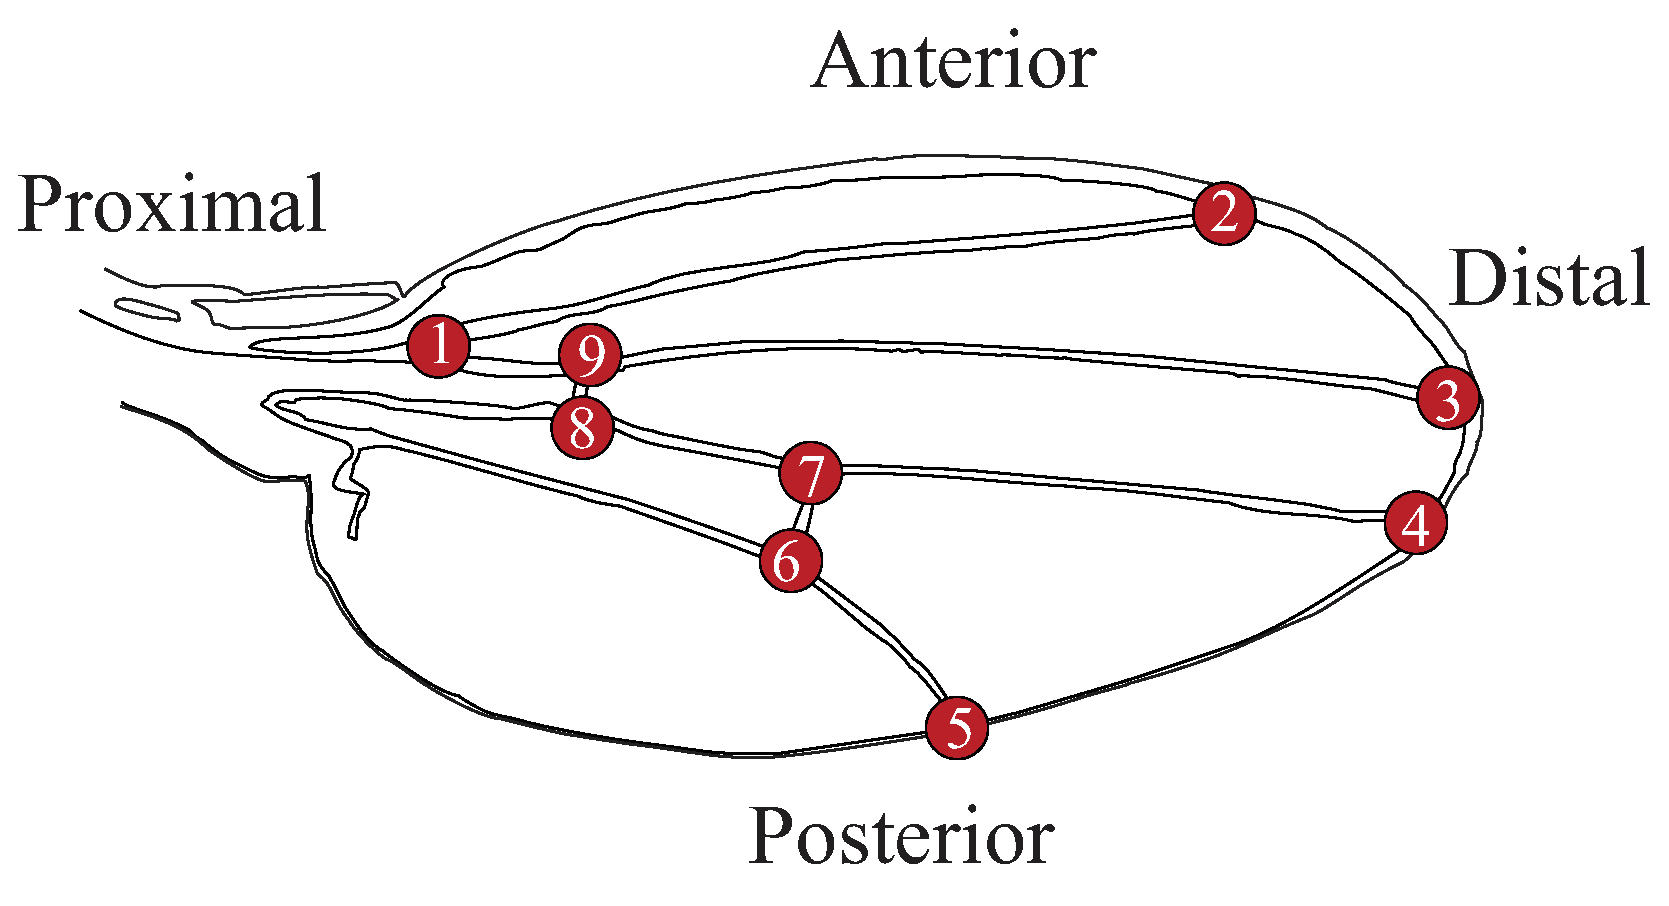
\includegraphics[width=0.7\textwidth]{Chp3_Multi/WingNineLM.eps}
\caption[Positions of the nine landmarks used to characterise wing shape.]{\textbf{Positions of the nine landmarks used to characterise wing shape.} Landmarks were: the proximal intersection of the radial vein (1), distal intersection of the radial vein (2), distal intersection of the medial vein (3), distal intersection of the cubital vein (4), distal intersection of the distal vein (5), the posterior (6) and the anterior (7) intersections of the posterior cross vein, and the posterior (8) and the anterior (9) intersections of the anterior cross-vein. Inter-landmark distance traits were described by their end-point landmarks (e.g., ILD1.2 was the distance between landmark1 and landmark 2), where the six traits analysed were: ILD1.2, ILD1.5, ILD2.5, ILD2.8, ILD3.7 and wing size characterised as centroid size (CS).} 
\label{fig:multi_WingNineLM}
\end{figure}
\newpage

%% Multivariate estimates of VL (M matrices)
\begin{figure}[htp]
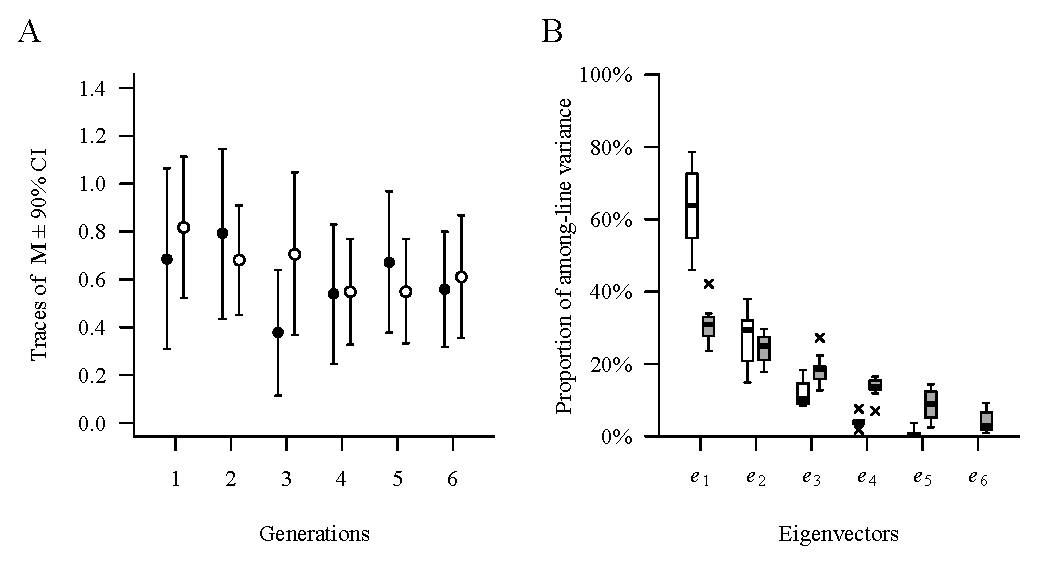
\includegraphics[width=1\textwidth]{Chp3_Multi/M_traceNeigs.eps}
\vspace*{-0.4cm}
\caption[The distribution of among-line variances in analyses of the 12 population six-trait \textbf{M}-matrices.]{\textbf{The distribution of among-line variances in analyses of the 12 population six-trait M-matrices.} (A) Matrices were estimated independently for each of the two population size treatments (small: solid circles; big: open circles), for each generation. The trace of the REML matrices (circle) and the 90\% confidence intervals estimated using 10,000 REML-MVN are plotted. (B) The distribution of multivariate versus univariate variances [Chapter 2] for the 12 populations. Open boxplots represent distribution across the 12 $\vec{M}$ in the proportion of among-line variance accounted for by each of the six eigenvectors (x-axis, $e_{1-6}$ ), calculated as the eigenvalue divided by the trace of the matrix. Note, a different combination of the six traits could represent the eigenvector associated with the most ($e_1$) versus least ($e_6$) for variance in each matrix, but the boxplots represent the distribution of how much (or how little) variance was explained by the largest to the smallest eigenvalue in each population. For comparison, the mutational variance in each individual trait (CS, ILD1.2, ILD1.5, ILD2.5, ILD2.8 and ILD3.7) was ranked from highest to lowest variance within each population, and their distribution in the 12 populations are also shown (grey boxplots). Note, a different trait might have ranked first versus sixth in each population, but this boxplot represents the variation among the 12 populations in the maximum to minimum individual trait variance. For each boxplot, the median of the distribution is shown as a black band, open boxes represent the interquartile range, whiskers represent 1.5 times the interquartile range, and estimates that fell outside this range are designated with crosses.}
\label{fig:multi_specM}
\end{figure}
\FloatBarrier

\begin{figure}[htp]
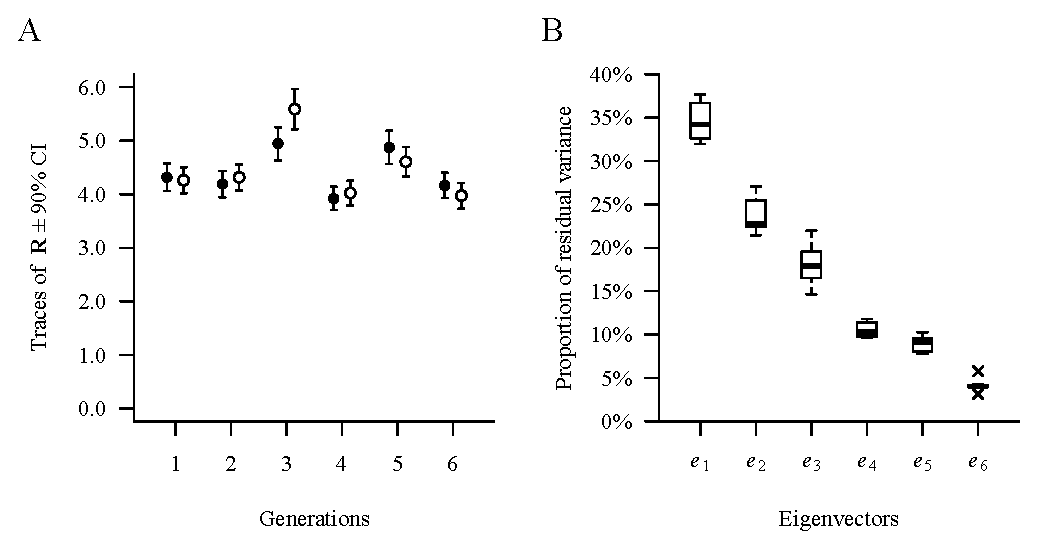
\includegraphics[width=1\textwidth]{Chp3_Multi/R_traceNeigs.eps}
\vspace*{-0.4cm}
\caption[The distribution of residual variances in analyses of the 12 population six-trait \textbf{R}-matrices.]{\textbf{The distribution of residual variances in analyses of the 12 population six-trait $\vec{R}$-matrices.} (A) Matrices were estimated independently for each of the two population size treatments (small: solid circles; big: open circles), for each generation. The trace of the REML matrices (circle) and the 90\% confidence intervals estimated using 10,000 REML-MVN are plotted. (B) The distribution of across the 12 $\vec{R}$ in the proportion of residual variance accounted for by each of the six eigenvectors (x-axis, $e_{1-6}$ ), calculated as the eigenvalue divided by the trace of the matrix. Note, similar to Figure~\ref{fig:multi_specM}, a different combination of the six traits could represent the eigenvector associated with the most ($e_1$) versus least ($e_6$) for variance in each matrix, but the boxplots represent the distribution of how much (or how little) variance was explained by the largest to the smallest eigenvalue in each population. }
\label{fig:multi_specR}
\end{figure}
\FloatBarrier

\begin{figure}[htp]
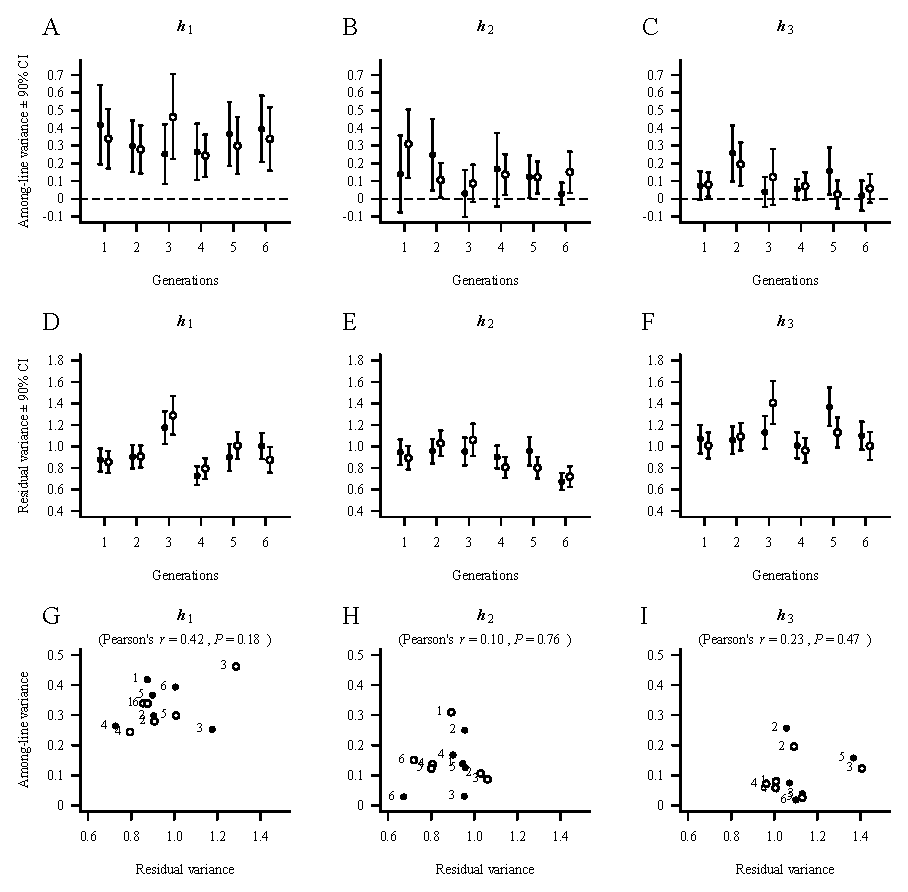
\includegraphics[width=1\textwidth]{Chp3_Multi/HvecsThruMnR.eps}
\vspace*{-0.4cm}
\caption[The among-line and residual variance associated with each of the three eigenvectors of the shared Krzanowski’s subspace.]{\textbf{The among-line and residual variance associated with each of the three eigenvectors of the shared Krzanowski’s subspace.} For each plot, the magnitude of the among-line variance (top panels: A, $h_1$; B, $h_2$; and C, $h_3$) and residual variance (middle panels: D, $h_1$; E, $h_2$; and F, $h_3$) in the specified multivariate axis of wing shape and size is plotted. The 90\% CI for the among-line variance ($V_L$) estimates and residual variances ($V_R$) were determined by projecting the Krzanowski’s subspace eigenvectors ($h_1$: $h_3$) through the 10,000 sets of twelve $\vec{M}$ and $\vec{R}$, respectively, generated using REML-MVN sampling. Within each plot, the populations are ordered by generation (x-axis), then by population size treatments (small: solid circles; large: open circles). The dashed lines indicate zero. Bottom panels (G, $h_1$; H, $h_2$; and I, $h_3$), the among-line variance (A:C) is plotted against the residual variance (D:F). Points represent population size treatments (small: solid circles; large: open circles) and are labelled by generation.}
\label{fig:multi_HvecsThruMnR}
\end{figure}
\FloatBarrier

\begin{figure}[htp]
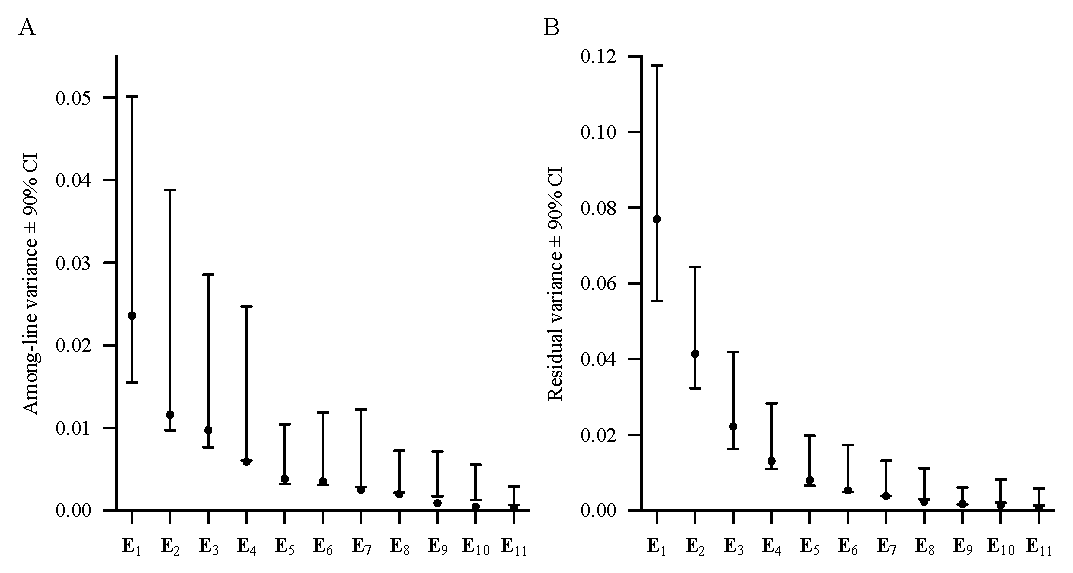
\includegraphics[width=1\textwidth]{Chp3_Multi/DaveFigTwoEigtensors.eps}
\vspace*{-0.4cm}
\caption[Among-line variance ($V_L$, A) and residual variance ($V_R$, B) accounted for by the first eleven non-zero eigentensors ($\vec{E}_k$).]{\textbf{Among-line variance ($V_L$, A) and residual variance ($V_R$, B) accounted for by the first eleven non-zero eigentensors ($\vec{E}_k$).} For the 90\% confidence intervals (CI) for the observed eigentensor estimates were determined using REML-MVN sampling of the respective $\vec{M}$ or $\vec{R}$ inverse Fisher Information matrices to estimate 10,000 $\vec{S}$ tensor matrices. Sampling distributions were obtained by projecting each of the eleven eigentensor eigenvectors separately through the 10,000 $\vec{S}$ tensor matrices to create a sampling distribution.}
\label{fig:multi_TwoEigTen}
\end{figure}
\FloatBarrier

\newpage
\begin{figure}[!htp]
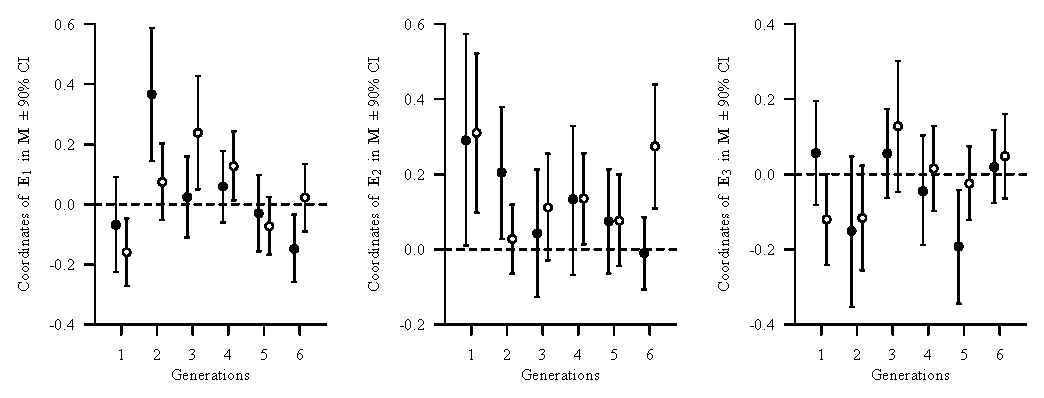
\includegraphics[width=1\textwidth]{Chp3_Multi/VL_Coords.eps}
\vspace*{-0.4cm}
\caption[Coordinates of the first three among-line ($V_L$) eigentensors ($\vec{E}_k$) through all twelve $\vec{M}$.]{\textbf{Coordinates of the first three among-line ($V_L$) eigentensors ($\vec{E}_k$) through all twelve $\vec{M}$.} The first three eigentensors accounted for 70\% of the variance in the eigentensor, $\Sigma_{\textbf{M}}$. The M matrices are ordered by generation (x-axis), then by population size treatments (small: solid circles; big: open circles). The 90\% CI for the coordinate estimates were determined using REML-MVN sampling of the 10,000 sets of twelve $\vec{M}$. Dashed horizontal line at zero for reference.}
\label{fig:multi_VLcoords}
\end{figure}
\FloatBarrier
\vspace{4cm}

\begin{figure}[!htp]
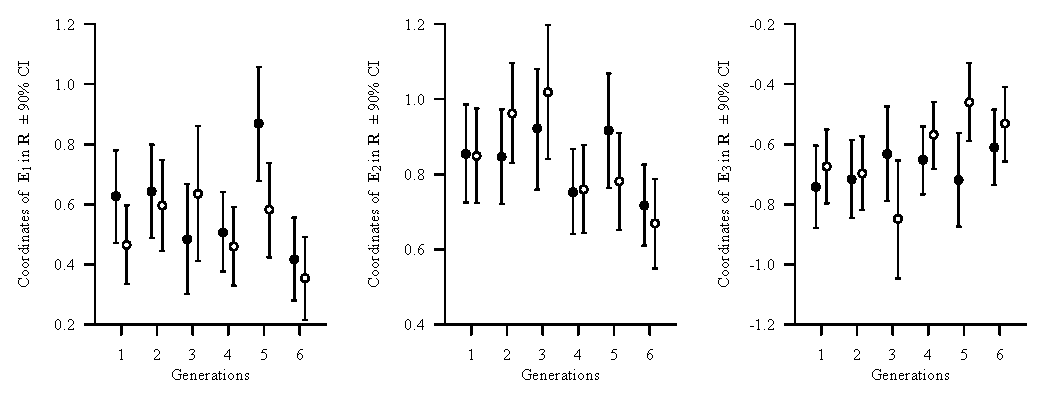
\includegraphics[width=1\textwidth]{Chp3_Multi/VLthruR_Coords.eps}
\vspace*{-0.4cm}
\caption[Coordinates of the first six among-line ($V_L$) eigentensors ($\vec{E}_k$) through all the twelve residual matrices, $\vec{R}$.]{\textbf{Coordinates of the first six among-line ($V_L$) eigentensors ($\vec{E}_k$) through all the twelve residual matrices, $\vec{R}$.} The R matrices are ordered by generation (x-axis), then by population size treatments (small: solid circles; big: open circles). The 90\% CI for the coordinate estimates were determined using REML-MVN sampling of the 10,000 sets of twelve $\vec{R}$.}
\label{fig:multi_VLthruRCoords}
\end{figure}
\FloatBarrier

\newpage
\begin{landscape}
\begin{figure}[htp]
\begin{center}
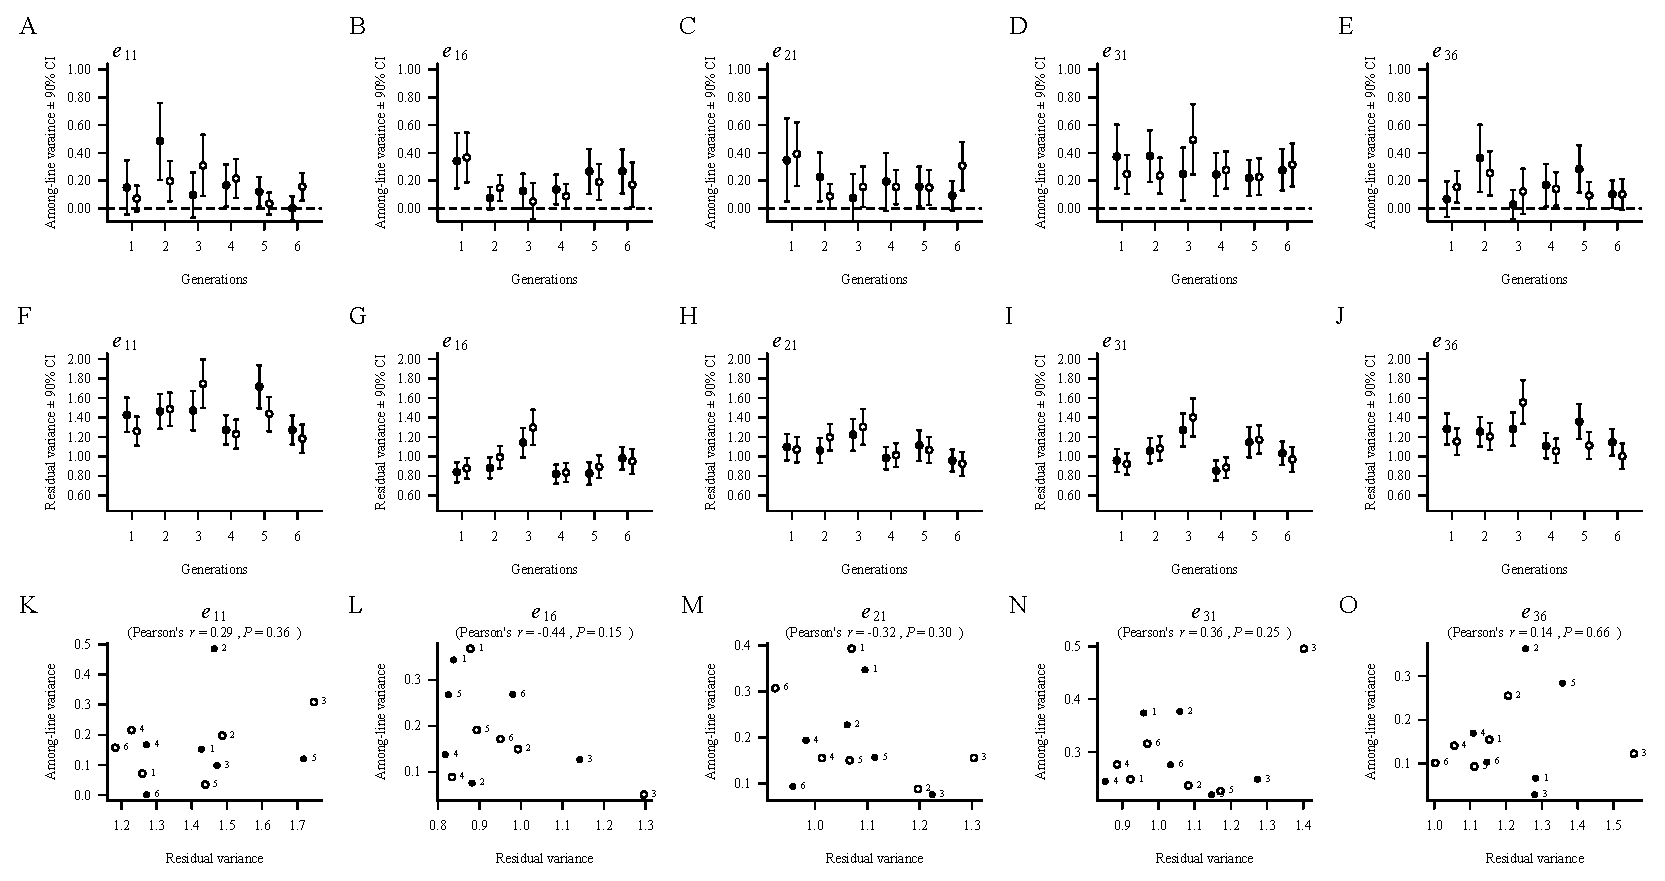
\includegraphics[width=1.39\textwidth]{Chp3_Multi/MajorEigentensorEigVecs.eps}
\end{center}
\caption[The among-line and residual variance associated with the major eigentensor eigenvectors ($e_{11}$, $e_{16}$, $e_{21}$, $e_{31}$, $e_{36}$) from the first three eigentensors for \textit{D. serrata} for six wing traits.]{\textbf{The among-line and residual variance associated with the major eigentensor eigenvectors ($e_{11}$, $e_{16}$, $e_{21}$, $e_{31}$, $e_{36}$) from the first three eigentensors for \textit{D. serrata} for six wing traits.} The eigentensor eigenvectors were projected through each $\vec{M}$ (top panels, A to E) as well as $\vec{R}$ (middle panels, F to J). Variances were estimated independently for each eigentensor eigenvector in each generation (x-axis) for each of the two population size treatments (small: solid circles; big: open circles). The 90\% CI were estimated using 10,000 REML-MVN samples of $\vec{M}$ and $\vec{R}$. Bottom panels (K:O), the among-line variance (A:E) is plotted against the residual variance (F:J). Points represent population size treatments (small: solid circles; large: open circles) and are labelled by generation.}
\label{fig:multi_mjEigTenEigVecs}
\end{figure}
\end{landscape}
\FloatBarrier



\begin{figure}[htp]
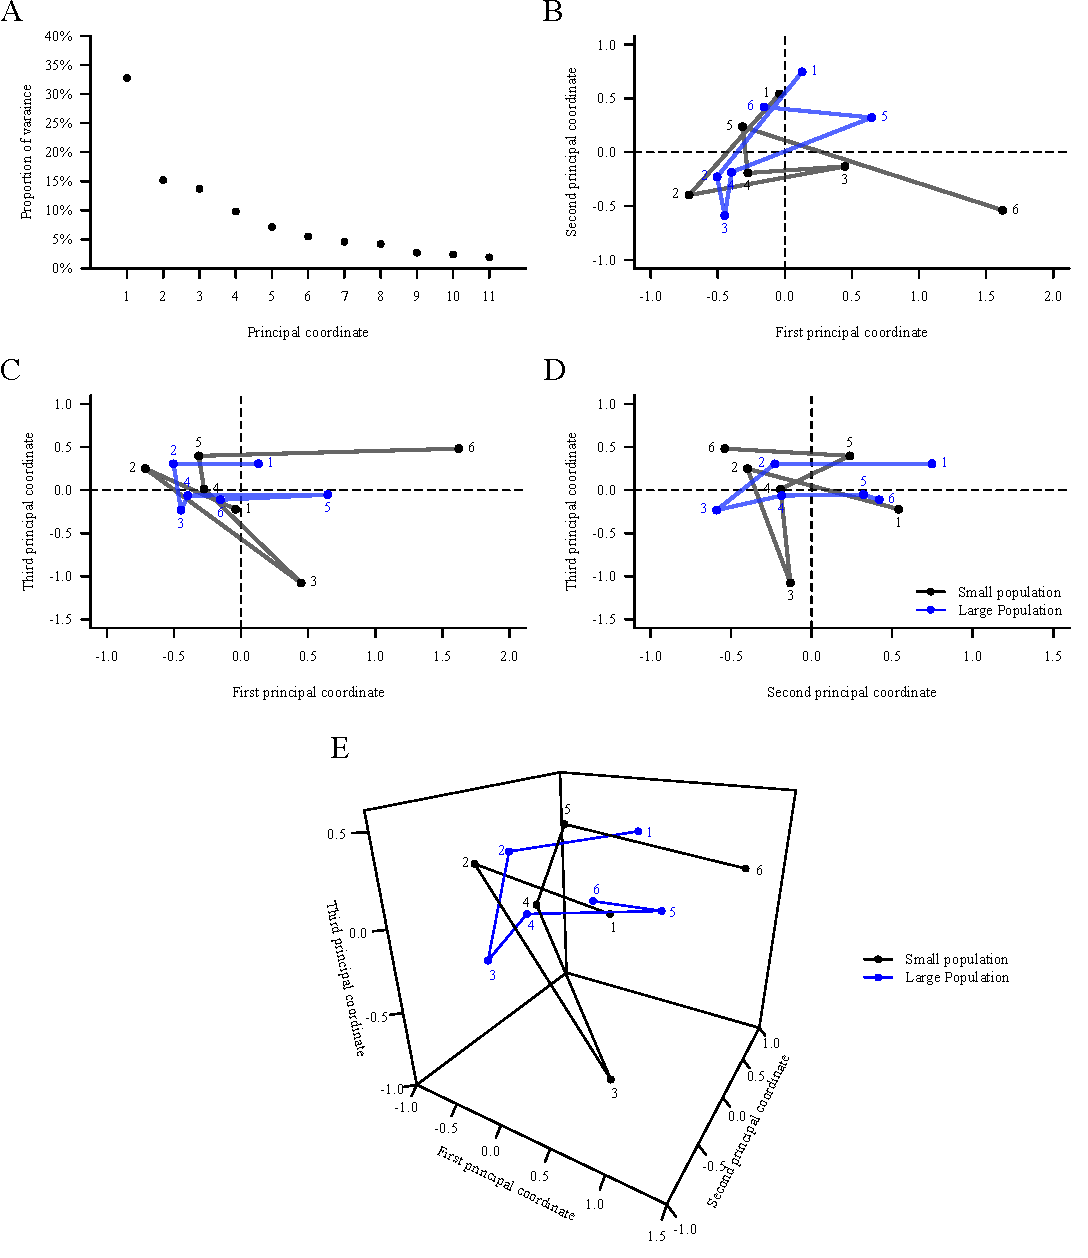
\includegraphics[width=1\textwidth]{Chp3_Multi/M_in_H_MittDist_3D.pdf}
\vspace*{-0.4cm}
\caption[Principal coordinates of the relative pairwise distances between the 12 $\vec{M}$.]{\textbf{Principal coordinates of the relative pairwise distances between the 12 $\vec{M}$.} (A) Proportion of variance accounted for by each of the principal coordinates. Bivariate scatter plots showing the projections between the first three principal coordinates of the 12 $\vec{M}$, account for varying amounts of variance: (A) first and second, 48.0\%; (B) first and third, 46.5\%; and, (C)~second and third, 28.9\%. Each point represents an individual $\vec{M}$, labelled by generation. (E) A trivariate scatter plot representation of bivariate plots B, C and D. Lines represent the trajectory through time for $\vec{M}$ in the small (black) and the large (blue) population size treatments.}
\label{fig:multi_Mitteroecker}
\end{figure}
\FloatBarrier

 

%%% eigenvectors of M
\newpage
\begin{table}[!htbp]
\renewcommand{\arraystretch}{0.9}
\caption[The variance associated with each of the eigenvectors of $\vec{M}$.]{\textbf{The variance associated with each of the eigenvectors of $\vec{M}$.} Eigenanalyses were performed separately for $\vec{M}$ in each population size treatment (small and large) for every generation. The eigenvalues (i.e., $\lambda$) are shown with 90\% CIs determined by projecting each eigenvector ($e_1$: $e_6$) through the 10,000 REML-MVN respective matrices. Eigenvalues with significant variance (lower 90\% CI does not overlap zero) are highlighted in bold. The vector loadings are provided in Table~\ref{tab:multi_suppEigVecM}.}
\label{tab:multi_Meigvals}
\begin{center}
\scriptsize
\begin{tabular}{>{\bfseries}cccccccc}
\toprule
\textbf{Treatment}& \textbf{Generation} & $e_1$& $e_2$& $e_3$& $e_4$& $e_5$& {$e_6$} \\
\midrule
Small & 1 & \bfseries{0.495} & \bfseries{0.102} & \bfseries{0.084} & 0.027 & 0.001 & -0.024 \\ 
 &  & 0.193; 0.798 & 0.014; 0.191 & 0.004; 0.165 & -0.036; 0.092 & -0.025; 0.027 & -0.073; 0.026 \\ [1.2ex]
 & 2 & \bfseries{0.506} & \bfseries{0.270} & 0.066 & 0.015 & -0.014 & -0.050 \\ 
 &  & 0.206; 0.804 & 0.133; 0.402 & -0.005; 0.136 & -0.013; 0.043 & -0.040; 0.012 & -0.091; -0.009 \\ [1.2ex]
 & 3 & \bfseries{0.276} & \bfseries{0.116} & 0.037 & 0.016 & -0.011 & -0.056 \\ 
 &  & 0.079; 0.472 & 0.032; 0.197 & -0.028; 0.102 & -0.039; 0.071 & -0.042; 0.020 & -0.138; 0.028 \\ [1.2ex]
 & 4 & \bfseries{0.279} & \bfseries{0.205} & 0.051 & 0.019 & 0.000 & -0.013 \\ 
 &  & 0.087; 0.471 & 0.029; 0.375 & -0.021; 0.121 & -0.008; 0.045 & -0.025; 0.025 & -0.044; 0.017 \\ [1.2ex]
 & 5 & \bfseries{0.429} & \bfseries{0.159} & \bfseries{0.114} & 0.029 & 0.010 & -0.070 \\ 
 &  & 0.213; 0.648 & 0.023; 0.297 & 0.008; 0.219 & -0.001; 0.060 & -0.015; 0.034 & -0.147; 0.007 \\ [1.2ex]
 & 6 & \bfseries{0.439} & \bfseries{0.093} & 0.047 & 0.021 & -0.004 & -0.037 \\ 
 &  & 0.238; 0.641 & 0.020; 0.165 & -0.001; 0.094 & -0.006; 0.049 & -0.044; 0.034 & -0.099; 0.025 \\ [1.2ex]
 \midrule
Large & 1 & \bfseries{0.446} & \bfseries{0.267} & \bfseries{0.070} & 0.033 & 0.008 & -0.007 \\ 
 &  & 0.211; 0.676 & 0.131; 0.406 & 0.007; 0.136 & -0.017; 0.082 & -0.013; 0.030 & -0.040; 0.026 \\[1.2ex] 
 & 2 & \bfseries{0.313} & \bfseries{0.215} & \bfseries{0.077} & 0.052 & 0.025 & 0.000 \\ 
 &  & 0.164; 0.460 & 0.073; 0.354 & 0.015; 0.138 & -0.006; 0.110 & -0.000; 0.050 & -0.020; 0.019 \\ [1.2ex]
 & 3 & \bfseries{0.529} & 0.144 & \bfseries{0.070} & 0.020 & -0.020 & -0.038 \\ 
 &  & 0.272; 0.792 & -0.014; 0.300 & 0.004; 0.137 & -0.009; 0.051 & -0.069; 0.029 & -0.115; 0.039 \\ [1.2ex]
 & 4 & \bfseries{0.303} & \bfseries{0.160} & \bfseries{0.101} & 0.020 & -0.006 & -0.029 \\ 
 &  & 0.144; 0.462 & 0.046; 0.273 & 0.030; 0.170 & -0.016; 0.058 & -0.025; 0.014 & -0.069; 0.010 \\ [1.2ex]
 & 5 & \bfseries{0.304} & \bfseries{0.163} & 0.059 & 0.023 & 0.001 & 0.000 \\ 
 &  & 0.151; 0.461 & 0.067; 0.257 & -0.019; 0.136 & -0.015; 0.060 & -0.054; 0.057 & -0.021; 0.020 \\ [1.2ex]
 & 6 & \bfseries{0.398} & \bfseries{0.129} & \bfseries{0.112} & \bfseries{0.022} & 0.004 & -0.055 \\ 
 &  & 0.194; 0.602 & 0.050; 0.209 & 0.010; 0.214 & 0.004; 0.039 & -0.035; 0.042 & -0.111; 0.002 \\ [1.2ex]
\bottomrule
\end{tabular}
\end{center}
\end{table}


%% Differences in covariances of M (Krzanowski's Subspaces)
\begin{table}[!htbp]
\caption[Eigenvalues ($\lambda$) and trait loadings for the first three major eigenvectors (\textit{\textbf{h}}$_{\textit{j}}$) of the shared Krzanowski's subspace, the H matrix.]{\textbf{Eigenvalues ($\lambda$) and trait loadings for the first three major eigenvectors (\textit{\textbf{h}}$_{\textit{j}}$) of the shared Krzanowski's subspace, the H matrix.}}
\label{tab:multi_Heigvals}
\begin{center}
\begin{tabular}{>{\bfseries}cS[table-format=2.2]S[table-format=2.2]S[table-format=2.2]}
\toprule
& {\textit{h}$_{\textit{1}}$} & {\textit{h}$_{\textit{2}}$} & {\textit{h}$_{\textit{3}}$}\\
\midrule
$\vec{\lambda}$ & 11.68 & 9.47 & 7.59 \\\cmidrule{2-4}
CS & 0.29 & 0.89 & -0.32\\
 ILD1.2 & -0.25 & 0.20 & 0.58\\
 ILD1.5 & -0.68 & 0.00 & -0.47\\
ILD2.5 & -0.20 & 0.07 & 0.20\\
 ILD2.8 & -0.15 & 0.32 & 0.55\\
 ILD3.7 & 0.57 &-0.26 & 0.08\\
\bottomrule
\end{tabular}
\end{center}
\end{table}


% =====Vector correlations ====%
\newpage
\begin{table}[!htbp]
\caption[Vector dot products between the first three major eigenvectors $h_j$ of the shared Krzanowski's subspace and major eigenvectors ($e_{kn}$) of the first three eigentensors ($\vec{E}_{1}$, $\vec{E}_{2}$ and $\vec{E}_{3}$) of $\Sigma_{\textbf{M}}$.]{\textbf{Vector dot products between the first three major eigenvectors $h_j$ of the shared Krzanowski's subspace and major eigenvectors ($e_{kn}$) of the first three eigentensors ($\vec{E}_{1}$, $\vec{E}_{2}$ and $\vec{E}_{3}$) of $\Sigma_{\textbf{M}}$.} Dot product measures the similarity of orientation between two vectors, where a value of zero indicates vectors are orthogonal, and a value of one indicates vectors are oriented in the same direction.}
\label{tab:multi_VecDotProd}
\begin{center}
\begin{tabular}{cS[table-format=2.2]S[table-format=2.2]S[table-format=2.2]S[table-format=2.2]S[table-format=2.2]}
\toprule
& {\textit{e}$_{\textit{11}}$} & {\textit{e}$_{\textit{16}}$} &
{\textit{e}$_{\textit{21}}$} & {\textit{e}$_{\textit{31}}$} & {\textit{e}$_{\textit{36}}$} \\
\midrule
$\textit{h}_{1}$  & 0.36	& 0.60	& -0.51 & 0.89	& -0.38\\
$\textit{h}_{2}$  & -0.45	& -0.37	& 0.83	& -0.15	& -0.63\\
$\textit{h}_{3}$  & 0.78	& -0.54	& 0.11	& 0.33	& 0.67 \\
\bottomrule
\end{tabular}
\end{center}
\end{table}

%======Main Eigentensor Eigenvector Loadings========
\begin{table}[!htbp]
\caption[Trait loadings for major eigenvectors ($e_{kn}$) of the first three eigentensors ($\vec{E}_{1}$, $\vec{E}_{2}$ and $\vec{E}_{3}$) of $\Sigma_{\textbf{M}}$.]{\textbf{Trait loadings for major eigenvectors ($e_{kn}$) of the first three eigentensors ($\vec{E}_{1}$, $\vec{E}_{2}$ and $\vec{E}_{3}$) of $\Sigma_{\textbf{M}}$.}}
\label{tab:multi_EigValLoadings}
\begin{center}
\begin{tabular}{>{\bfseries}cS[table-format=2.2]S[table-format=2.2]S[table-format=2.2]S[table-format=2.2]S[table-format=2.2]}
\toprule
& {\textit{e}$_{\textit{11}}$} & {\textit{e}$_{\textit{16}}$} & {\textit{e}$_{\textit{21}}$} & {\textit{e}$_{\textit{31}}$} & {\textit{e}$_{\textit{36}}$} \\
\midrule
$\vec{\lambda}$ & 0.80 & -0.57 & 0.93 & 0.43 & -0.80 \\ \cmidrule{2-6}
CS & -0.07 & -0.28 & 0.62 & 0.21 & -0.46 \\ 
ILD1.2 & -0.77 & -0.03 & 0.27 & -0.59 & -0.43 \\ 
ILD1.5 & 0.01 & -0.56 & 0.30 & -0.58 & 0.55 \\ 
ILD2.5 & -0.12 & 0.36 & 0.22 & -0.12 & 0.01 \\ 
ILD2.8 & -0.61 & 0.14 & 0.13 & -0.36 & -0.54 \\ 
ILD3.7 & 0.14 & 0.68 & -0.62 & 0.37 & -0.11 \\
\bottomrule
\end{tabular}
\end{center}
\end{table}

